\PassOptionsToPackage{dvispnames, table}{xcolor}
\documentclass[aspectratio=169, hyperref={colorlinks=true}]{beamer}
\usepackage[beamer]{prettytex/base}
\usepackage{prettytex/math}
\usepackage{prettytex/gfx}
\usepackage[backend=biber, citestyle=numeric, bibstyle=numeric, hyperref=true, sorting=none, maxbibnames=99]{biblatex}
\usepackage{csquotes}
\usepackage{fontawesome}
\addbibresource{../literature/sources.bib}
\renewcommand{\figureloc}{../figures}  % for tikzfigures
\usetheme{oxonian}

\title{General Kernel Spectral Methods for Equilibrium Measures \\ \normalsize An MMSC Dissertation Project}
\titlegraphic{
\includegraphics[width=2cm]{theme/logos/ox-circle.eps}}
\author{Peter Julius Waldert}
\institute{Mathematical Institute \\ University of Oxford}
\date{$22^{\rm nd}$ of May, 2023}

\begin{document}
  {\setbeamertemplate{footline}{}\frame{\titlepage}}

  \section{Intro}
  \begin{frame}{Problem Setting}
    \begin{itemize}
      \item Find the Equilibrium Distribution $\rho(\vec{x})$ of a Many-Particle-System.
    \end{itemize}
    \begin{figure}[H]
      \centering
      \begin{subfigure}[t]{0.5\textwidth}
        \centering
        \inputtikz{problem-setting}
        \caption*{$N = 8$ particles interacting with one another through the potential $K(r)$.}
      \end{subfigure}
      \hfill
      \begin{subfigure}[t]{0.49\textwidth}
        \centering
        \scalebox{0.68}{\inputtikz{potential-function}}
        \caption*{Plot of attractive-repulsive potential functions $K(r) = \frac{r^\alpha}{\alpha} - \frac{r^\beta}{\beta}$ for different $\alpha, \beta$.}
      \end{subfigure}
    \end{figure}
  \end{frame}

  {
  \setbeamertemplate{footline}{}
  \begin{frame}{Project Motivation and Goal}
    \vspace{0.4cm}
    \begin{itemize}
      \item Interactions through (power-law) Attraction-Repulsion Potentials\footnote{If the repulsive term is stronger (so $\beta > \alpha$), there is no equilibium distribution as particles simply continue repelling each other out to infinity.}
            $$K(r) = \frac{r^\alpha}{\alpha} - \frac{r^\beta}{\beta}\quad \text{ with parameters } \quad \alpha, \beta \in \R \backslash \{0\}\,.$$
      \item Each particle $i=1, ..., N$ at position $\vec{x_i} \in \R^d$ and time $t \in \R^+$ follows
            $$\frac{\dd^2 \vec{x_i}}{\ddt^2} = f\left(\norm{\frac{\dd \vec{x_i}}{\ddt}}_2\right) \frac{\dd\vec{x_i}}{\ddt} - \frac{1}{N} \sum_{j=1, i\neq j}^{N} \nabla K\left(\norm{\vec{x_i} - \vec{x_j}}_2\right)\,,$$
            for reference see, for example, \parencite{2020-power-law-kernels, 2021-arbitrary-dimensions}.
            For now, we only consider the case without an external potential $V(\vec{x})$.
    \end{itemize}
  \end{frame}
  }

  \begin{frame}{Simulation Results}
    \begin{figure}
      \centering
      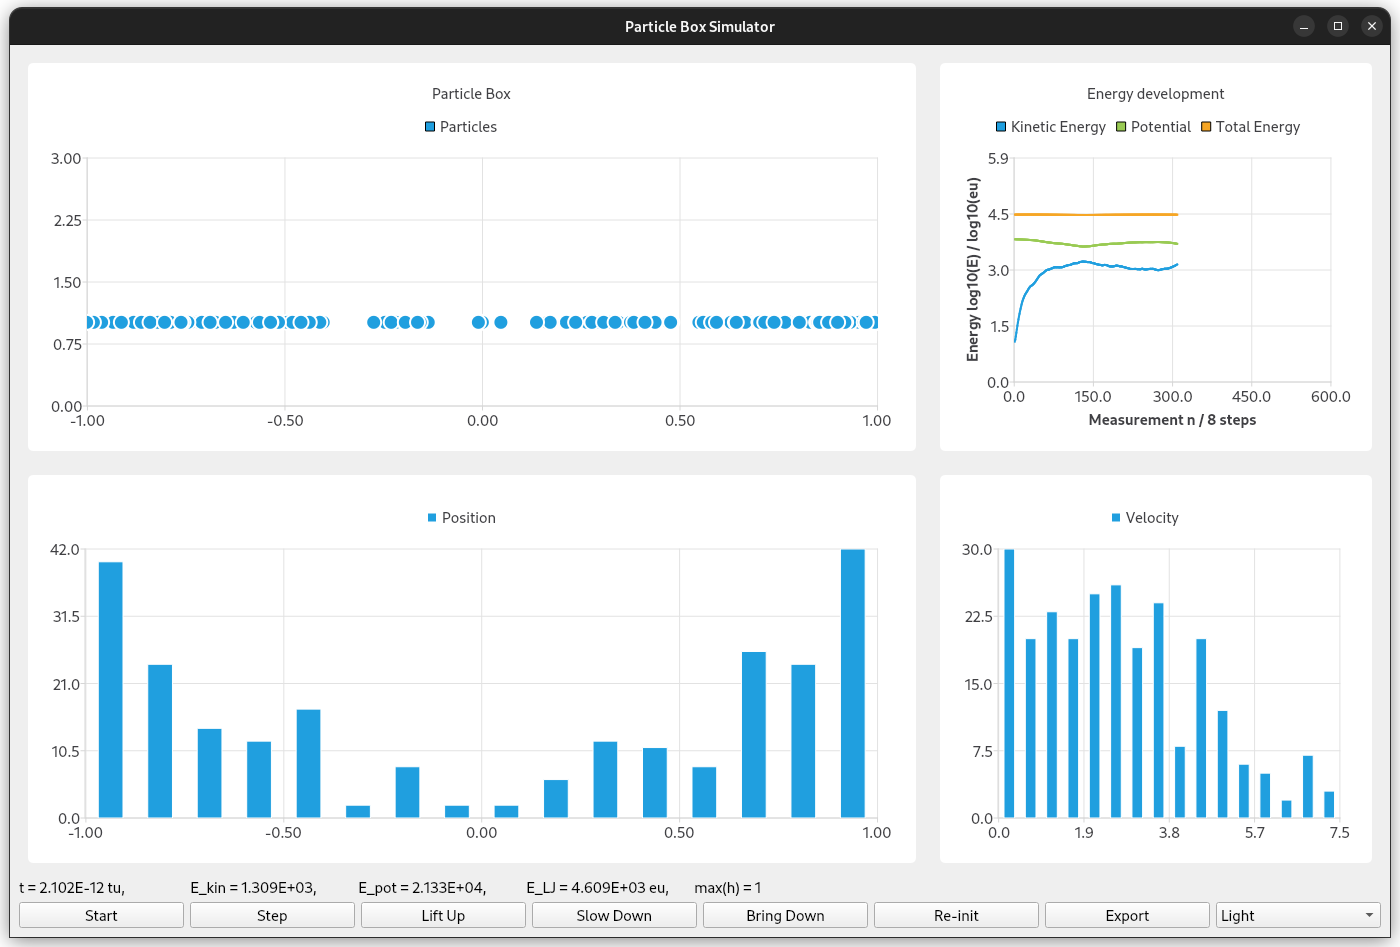
\includegraphics[width=0.64\linewidth]{figures/screenshot5.png}
      \caption*{The positional distribution approached by $N = 250$ particles.}
    \end{figure}
  \end{frame}

  \begin{frame}{An Integral Equation}
    \vspace{0.4cm}
    The total potential energy of an $N$-particle system is then given by
    $$E = \sum_{i=1}^{N} \sum_{j=1, j \neq i}^{N} K\left(\norm{\vec{x_i} - \vec{x_j}}_2\right)\,,$$
    which, in the continuous limit as $N \goesto \infty$, becomes
    $$E = \frac{1}{2} \iint K\left(\norm{\vec{x} - \vec{y}}_2\right) \,\dd\rho(\vec{x})\,\dd\rho(\vec{y})\,,$$
    where $\dd\rho = \rho(\vec{x})\dd\vec{x}$ is a measure (the equilibrium distribution) chosen such that
    $$M = \int \dd\rho = \int_{\supp(\rho)} \rho(\vec{x}) \,\dd\vec{x} = 1\,.$$
  \end{frame}

  \begin{frame}{Spectral Methods}
    \begin{itemize}
      \item In order to find $\rho(\vec{x})$, we consider the following ansatz
            $$\rho(\vec{x}) = \sum_{n=0}^{\infty} c_n P_n^{(a,b)}(\vec{x})\,,\quad c_n \in \R\,,$$
            with which we construct a spectral method for the numerical solution of the above integral equation.
      \item Minimization routine of $E$ over coefficients in $\rho$, as a subroutine of outer minimisation over the bounds of the box (simpler case: use $[-r, r]$, $r \in \R^+$).
      \item By construction, we find that we do not need an iterative approach for the inner optimisation routine.
      \item The outer minimisation can be performed using known methods from continuous optimisation.
    \end{itemize}
  \end{frame}

  \begin{frame}{Complete Polynomial Basis}
    Jacobi polynomials $P_n^{(a,b)}(x)$ are orthogonal on $[-1,1]$ w.r.t. the weight function
    \begin{equation*}
      w^{(a,b)}(x)=(1-x)^a (1+x)^b\,,
    \end{equation*}
    so they satisfy
    \begin{align*}\label{eq:orthogonalityconditionJacobi}
      \int_{-1}^1(1-x)^a(1+x)^bP_n^{(a,b)}P_m^{(a,b)}\,\ddx = \frac{2^{a+b+1} \Gamma (a+n+1) \Gamma (b+n+1)}{n! (a+b+2 n+1) \Gamma (a+b+n+1)} \delta_{n,m}\,,
    \end{align*}
    with $a	,b>-1$, which uniquely determines $P_n^{(a,b)}(x)$. The special case of $a=b$ corresponds to the ultraspherical or Gegenbauer polynomials, while the case $a=b=0$ corresponds to the Legendre polynomials \cite{2018-nist}.

    \begin{itemize}
      \item This basis yields a \textbf{sparse}, and in particular, \textbf{banded} operator.
    \end{itemize}
  \end{frame}

  \begin{frame}{Results from the Spectral Solver}
    \vspace{0.4cm}
    Using the spectral method, we try to immediately solve for the distribution function in the continuous limit (here, $d = 1$ dimension).
    \vspace{0.4cm}

    \begin{columns}
      \begin{column}{0.5\textwidth}
        \begin{figure}[H]
          \centering
          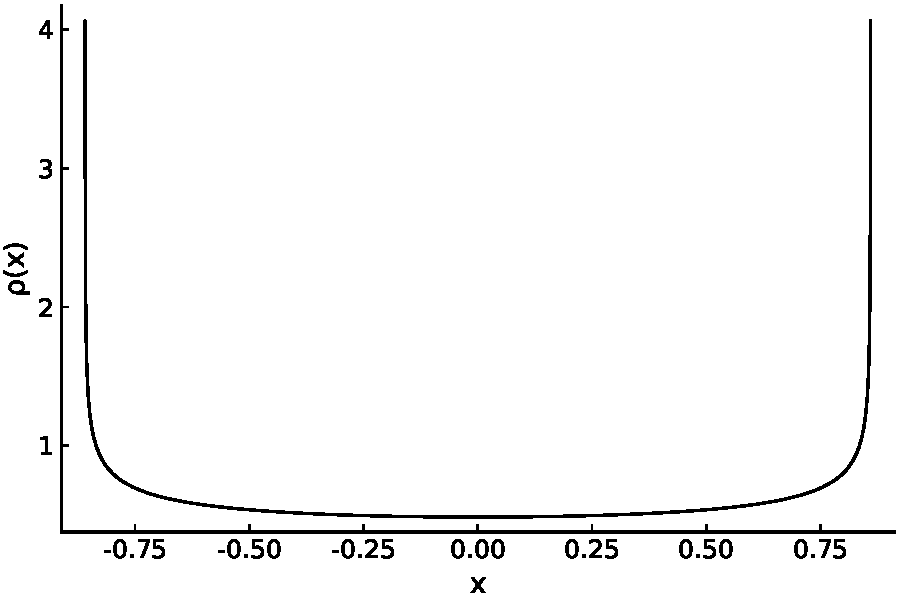
\includegraphics[width=0.9\linewidth]{figures/a2b1-5-measure.pdf}
          \caption*{Equilibrium distribution $(\alpha,\beta) = (2, 1.5)$ \cite{2020-power-law-kernels}.}
        \end{figure}
      \end{column}
      \begin{column}{0.5\textwidth}
        \begin{figure}[H]
          \centering
          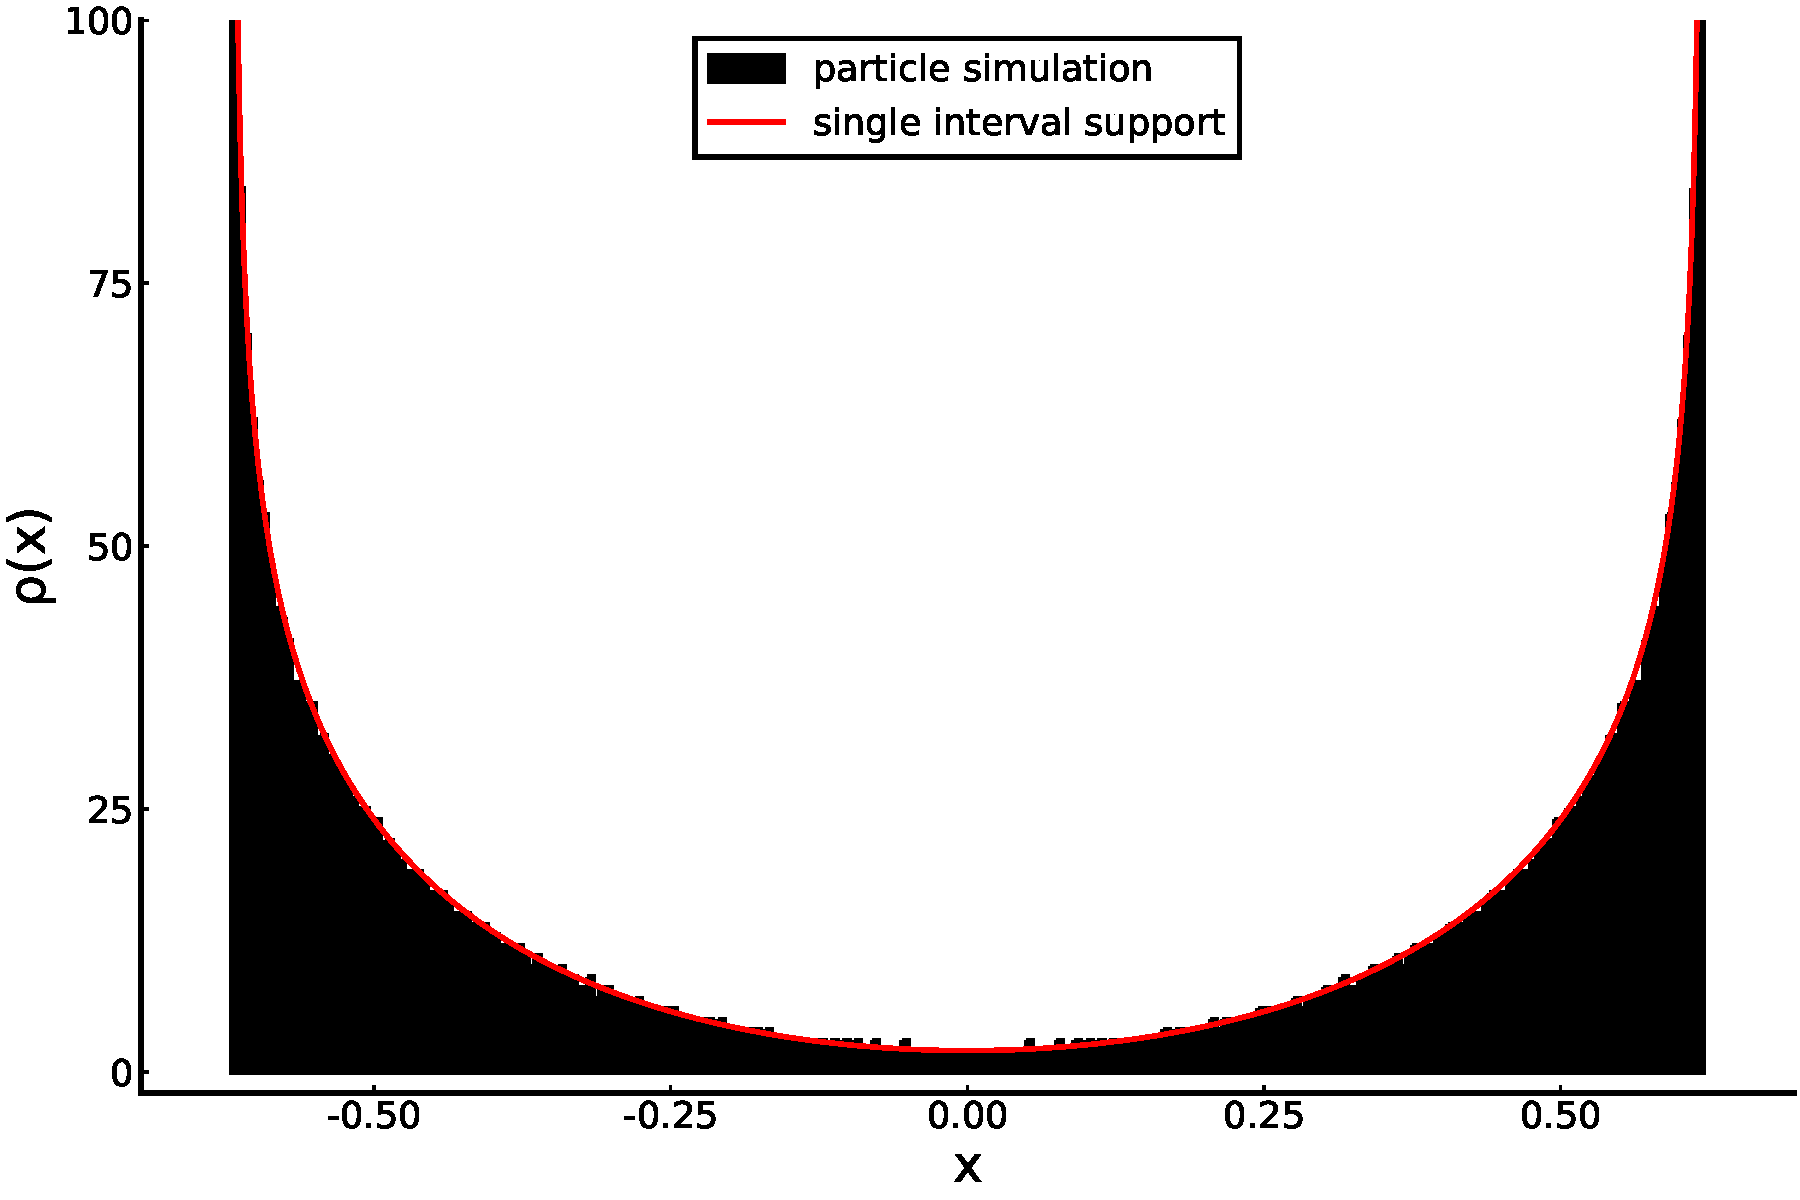
\includegraphics[width=0.9\linewidth]{figures/a35b16_supplement_3k.pdf}
          \caption*{Equilib. distribution $(\alpha, \beta) = (3.5, 1.6)$ \cite{2020-power-law-kernels}.}
        \end{figure}
      \end{column}
    \end{columns}
  \end{frame}

  \begin{frame}{Two Dimensional Results}
    \vspace{0.4cm}
    The same is possible for $d = 2$ or more dimensions.
    \begin{figure}[H]
      \centering
      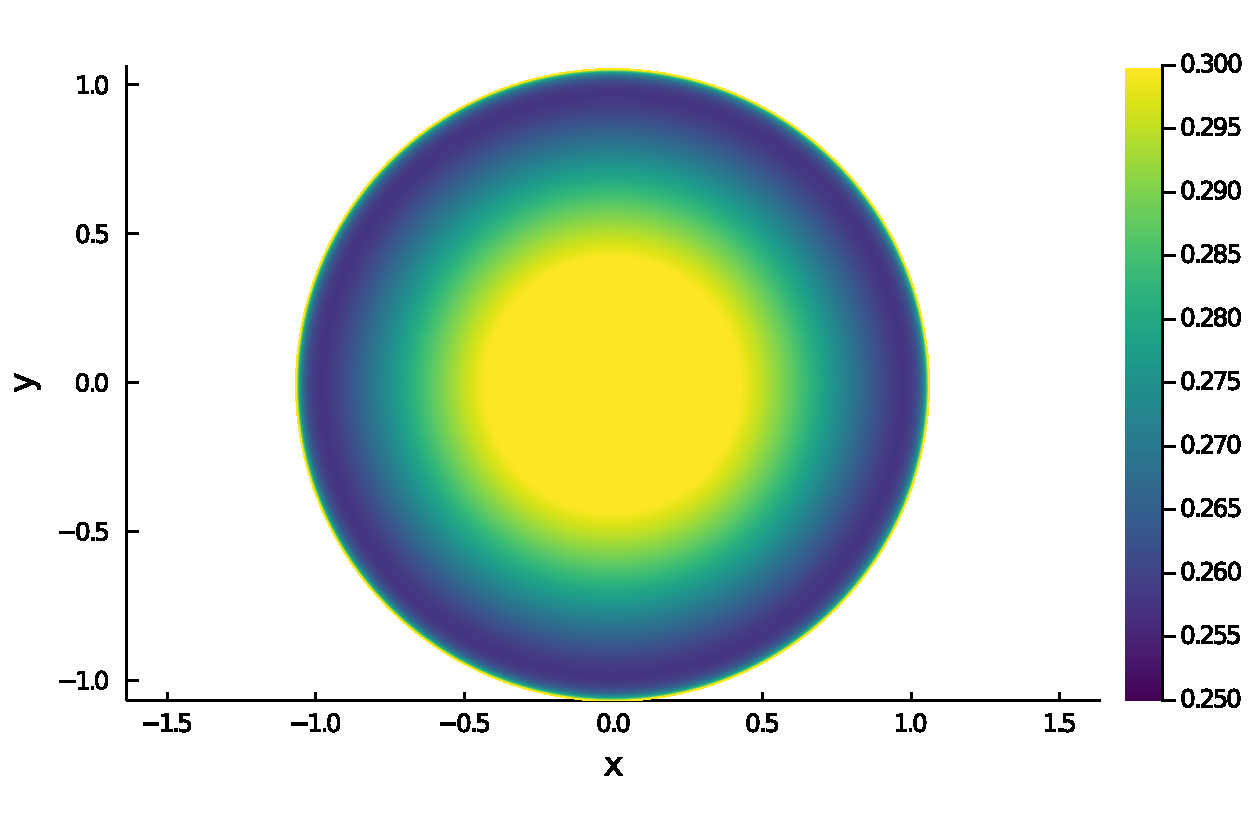
\includegraphics[width=0.5\linewidth]{figures/spectral-solution-2d.pdf}
      \caption*{The radially symmetric equilibrium distribution $\rho(\vec{x})$ for $\alpha = 1.2$, $\beta = 0.1993$ in $d = 2$ dimensions, obtained using a spectral method \cite{2021-arbitrary-dimensions}.}
    \end{figure}
  \end{frame}

  \begin{frame}{Upcoming Work}
    In this MMSC dissertation project, we will:
    \begin{itemize}
      \tightlist
      \item Establish theory behind spectral methods in the Jacobi basis.
      \item Use kernel expansions to construct an equilibrium measure method on $[-1, 1]$.
      \item Numerically solve for $\rho(\vec{x})$ using a fully implemented spectral solver\footnote{This is the first numerical method for particle distribution problems!}.
      \item Implement a particle simulator for the same kernel $K$ (mostly done).
      \item Compare results of the two methods and analytic solutions of special cases \cite{2014-explicit-flock-solutions-for-quasi-morse-potentials}.
    \end{itemize}
    Further goals include:
    \begin{itemize}
      \tightlist
      \item Considering the $d$-dimensional unit ball domain ($d > 1$).
      \item Optionally: Considering external potentials $V(\vec{x})$.
      \item Optionally: Extending to l-Morse potentials $K(r) = C_1 \e^{r / l_1} - C_2 \e^{r / l_2}$.
    \end{itemize}
  \end{frame}

  \begin{frame}{}
    Questions?
  \end{frame}

  \begin{frame}[allowframebreaks]
    \frametitle{Bibliography}
    \printbibliography[heading=bibnumbered]
  \end{frame}
\end{document}
